\chapter{Community concept}
\label{CommunityConcept}
%I dette kapitel skal konceptet bag TonePrint communitiet forklares med udgangspunkt i at der tilsidst skal tages et valg af hvilken det vi skal hjælpe med at udvikle.\\
Based on the description of TC Electronics development process in \autoref{InterviewConclusion}, the current task is to develop conceptual models, which describes the functionalities and use cases of the TonePrint Community. The scope of this phase is to discover which tasks that lay ahead the development of the TonePrint Community, while focusing on user involvement and user experience. \\

\section{Conceptual model}
\label{ConceptualModel}
In \parencite[][17]{PDF:Henderson2012} a conceptual model is descried  as "\textit{A high-level description of an application. It enumerates all concepts in the application that users can encounter, describes how those concepts relate to each other, and explains how those concepts fit into tasks that users perform with the application}".\\
In order to create the conceptual model of the TonePrint Community, some decisions have to be taken about functions, features and interactions, which hasn't been made on a business level yet. These decisions are therefore not fixed, in term of the final product, but will serve its purpose for this project. The decisions are based on the interviews in \autoref{ThemanticAnalysis} and reflects ideas and opinions from the development team.

\subsection{The TonePrint Concept model}
\label{TonePrintConceptualModel}
When creating the conceptual model we need to look at the task domains in which the user till perform activities to reach their goal. Different users have different purposes for using the community and therefore will there be more than one task domain to consider, while designing the community. \\
At first we look at the different groups of users for the TonePrint concept, as described in (\footnote{Appendix or analysis of interview}). On \autoref{fig:TonePrintUserConpt} it's depicted how users of the TonePrint concept are categorized into three groups, Pedal only users, TonePrint Users and TonePrint creators. The 'Pedal only users' are the users whom own a TonePrint pedal, but doesn't use the TonePrint functionalities of the pedal and just are using it as a regular pedal. We define the TonePrint Users as those who use the TonePrint concept to find and beam Artist TonePrints to their pedals. These users are therefore connected to the Artist Library of the TonePrint application. We define the TonePrint Creators as those whom uses the TonePrint concept to create User TonePrints, which they can use with their pedals. These users are therefore connected to the Editor and the User TonePrint Library. The connecting arrow between TonePrint Users and Creators on \autoref{fig:TonePrintUserConpt} indicates that these users isn't necessary different people, but might be the same user using the system differently. 

\begin{figure}[H]
	\centering
	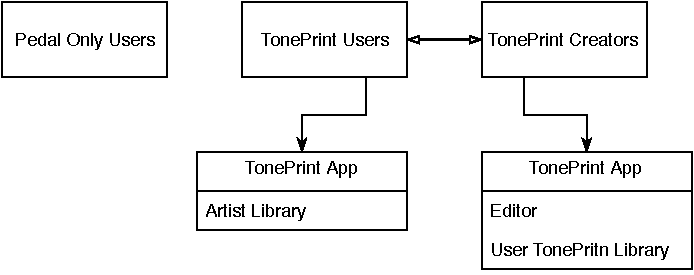
\includegraphics[width=0.85\textwidth]{TonePrintConcept.pdf}
	\caption{This illustrates the different groups of users of the TonePrint concept}
	\label{fig:TonePrintUserConpt}
\end{figure}

The definition of the different user groups of the TonePrint concept will also be applied to the concept of the TonePrint Community, however are the 'Pedal Only Users' neglected in future models. This is because they aren't using the TonePrint functions and thereby don't have any use of the TonePrint Community. The features listed in \autoref{tab:ListOfCommunityFeatures} are suggested to accommodate both the TonePrint users and creators in the community. The features are based on the ideas and suggestions from the interview with development team in \autoref{ThemanticAnalysis}.

\begin{table}[H]
	\centering
\begin{tabular}[width=\textwidth]{c|l}
\textbf{Ref. nr} & \textbf{Features} \\ \hline
1 & Uploading TonePrints \\ \hline
2 & Categorize by tags \\ \hline
3 & TonePrint description \\ \hline
4 & Search \\ \hline
5 & Rate TonePrint \\ \hline
6 & Subscribe to users \\ \hline
7 & Recommendations \\ \hline
8 & User profile \\ \hline
\end{tabular}
\caption{The left column contains the number which is used to refer to the feature in the right column}
\label{tab:ListOfCommunityFeatures}
\end{table}

The features 1, 2 and 3 in \autoref{tab:ListOfCommunityFeatures} are all closely related and accommodates especially the task domain of the TonePrint Creators. The feature of uploading features are simply to enable user to upload TonePrints to the community, that they have created with the editor. This feature covers the main function requested by the users which is the ability to share TonePrint with each other. \\
Feature 2, Categorizing by tags refers to the idea of letting users use tags to categorize the TonePrint they have uploaded. The purpose of these tags are to easily allow other users to identify which categories the TonePrint belongs to, which also enable users to find the discover tonePrints by searching on different tags/categories.\\
Feature 3, TonePrint description allows the creator of a TonePrint to write about the TonePrint, similar to the descriptions of the Artist TonePrints in the current TonePrint application. The description might contain information about the parameter settings, inspiration, self-promoting text or likewise. \\
Feature 4 is a search function which users can use to search for TonePrints, either by name, tag, artist, pedal or likewise. As one mentions in the interview it's essential to make this a proper search engine(\footnote{Tjek}). The current search functionality for the TonePrint application, which only is idle for android, is very limited and wouldn't be sufficient, as mentioned in \autoref{Heuristic_Results}. \\
Feature 5, the Rate TonePrint feature, is based on the idea of letting TonePrint users, whom have tried a creators TonePrints, rate the TonePrints. This rating could work as a motivation for creators to create more TonePrints, while it as the same time gives the TonePrint users the opportunity to see how much other users like the TonePrint. \\
Feature 6, Subscribe to users, are a feature which enables users to follow other users. A user could for instance have tried a TonePrint created by a certain other user and like it to a degree of which he want's to see which other TonePrints that user have created, and wants to be notified when new ones are created.\\
Feature 7, Recommendation, this feature is suggested to help users find and explore TonePrints. This could be recommendations like, "People who like this TonePrint also like these", "These are the highest rated TonePrints for your pedals" or "These TonePrints will at something new" etc.\\
Feature 8, Community Profile, is a feature which sums it all up. This profile is going to be a 'Front Page' for the users containing their own TonePrints, their recommendations, the TonePrints of those they subscribe to and the option to make a personal description and link to personal youtube, soundcloud or likewise sites, as a self-promoting feature.\\
\\
How the eight features above works on a detailed and technical level won't be a concern at the conceptual model. The goal of the conceptual model is to explain the relationship between functions, which can be used to perform the activities necessary for the user to reach a goal \parencite{Henderson2012}(Kilden skal opdateres så der er et kapitel mere med).


\subsection{Community Model}
\label{CommunityModel}
\footnote{(Opdater billede, spell check, add follower list, User library -> Profile Library, Community -> Community platform, Connection from editor to User TonePrint)}
The Toneprint communitys conceptual model consists of several concepts, which includes the already mentioned features \autoref{tab:ListOfCommunityFeatures}, which works together to accommodate the users needs. The conceptual model of the TonePrint Community is illustrated on \autoref{fig:CommunityConceptualModel}.\\

\begin{figure}[H]
	\centering
	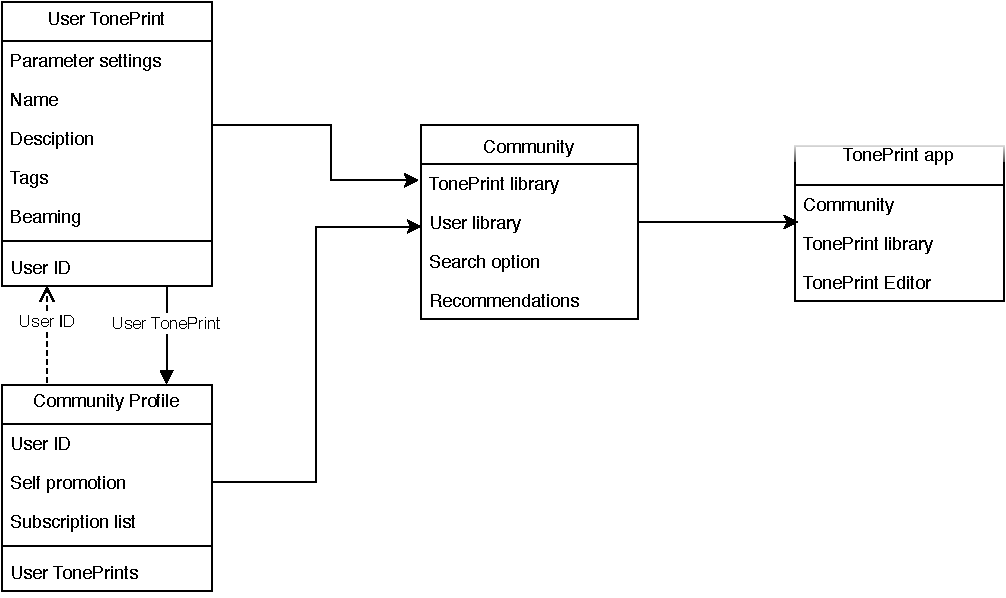
\includegraphics[width=0.90\textwidth]{CommunityFirstDraft.pdf}
	\caption{Illustration of the relationships of the concepts that makes up the Communities conceptual model}
	\label{fig:CommunityConceptualModel}
\end{figure}

At first there is the User TonePrint concept which contains: Parameter settings for the TonePrint. The name of the TonePrint. A description of the TonePrint (Feature 3 in \autoref{tab:ListOfCommunityFeatures}). Tags that categorize the TonePrint (Feature 2 in \autoref{tab:ListOfCommunityFeatures}). The beaming functionality (\footnote{Skal det med}). And lastly User ID, which is inherited from the Community Profile, which identifies the creator. This concepts differs from the original User TonePrint concept by adding the Description, tags and User ID, which all are new additions which aims to accommodate and ease the use of the Community. The User TonePrints are uploaded to the Communitys TonePrint library, for all user to find. It's also uploaded to the users own Community Profile so it's always easy accessible.\\
Secondly there is the Community Profile (Feature 8 in \autoref{tab:ListOfCommunityFeatures}) which contains: User ID that is used to identify the profile. Self-promotion which could include self description or links to other personal sites etc. Subscription list, which is a list of the user whom the user are subscribing to. Follower list, which is a list of those whom subscribe to the user. And lastly the User TonePrints which is a list of the users self created TonePrints. The Community Profile is crucial to shape the concept of including the users into a community, instead of just having a simple Upload/Download site. Some of the idea of self-promotion stems from the workshop in (Jespers kilde) and is also mentioned in (ref til interview/tema). The Community profile will work as a starting point for users when interacting with the Community.\\
Thirdly there's the Community platform which contains: The TonePrint library which give access to use and rate all the uploaded TonePrints (Feature 5 in \autoref{tab:ListOfCommunityFeatures}). The Profile library give access to visit all of the Community Profiles and subscribe to them (Feature 6 in \autoref{tab:ListOfCommunityFeatures}). Search option (Feature 4 in \autoref{tab:ListOfCommunityFeatures}) is simply a function which help user find the TonePrint they are looking fore. Recommendations which is described above(Feature 7 in \autoref{tab:ListOfCommunityFeatures}). The Community Platform sums up all of the features and concepts which shapes the TonePrint Community concept, by using both the User TonePrint concept and the Community Profile concept.\\
Lastly there is the concept of the TonePrint application which contains: The Community Platform, which represent all of the features and concepts of the TonePrint Community. The TonePrint library represent both the User TonePrint library and the Artist TonePrint library, first described in \autoref{TonePrintSoftware}, and seen in \autoref{fig:TonePrintUserConpt}. The TonePrint Editor, which is used to create the User TonePrints, which is described in \autoref{TonePrintSoftware} and seen in \autoref{fig:TonePrintUserConpt} (\footnote{tjek om vi siger det vi vil bruge i der hvor vi referer til}). The only change in the TonePrint application concept is the addition of the Community concept. As see in (Finde ref fra interview) does all of the interviewees agree upon letting the community be a part of the TonePrint application, however might there still be some disagreement to what extend it's to be included. 

\subsection{Use case}

\begin{figure}
	\centering
	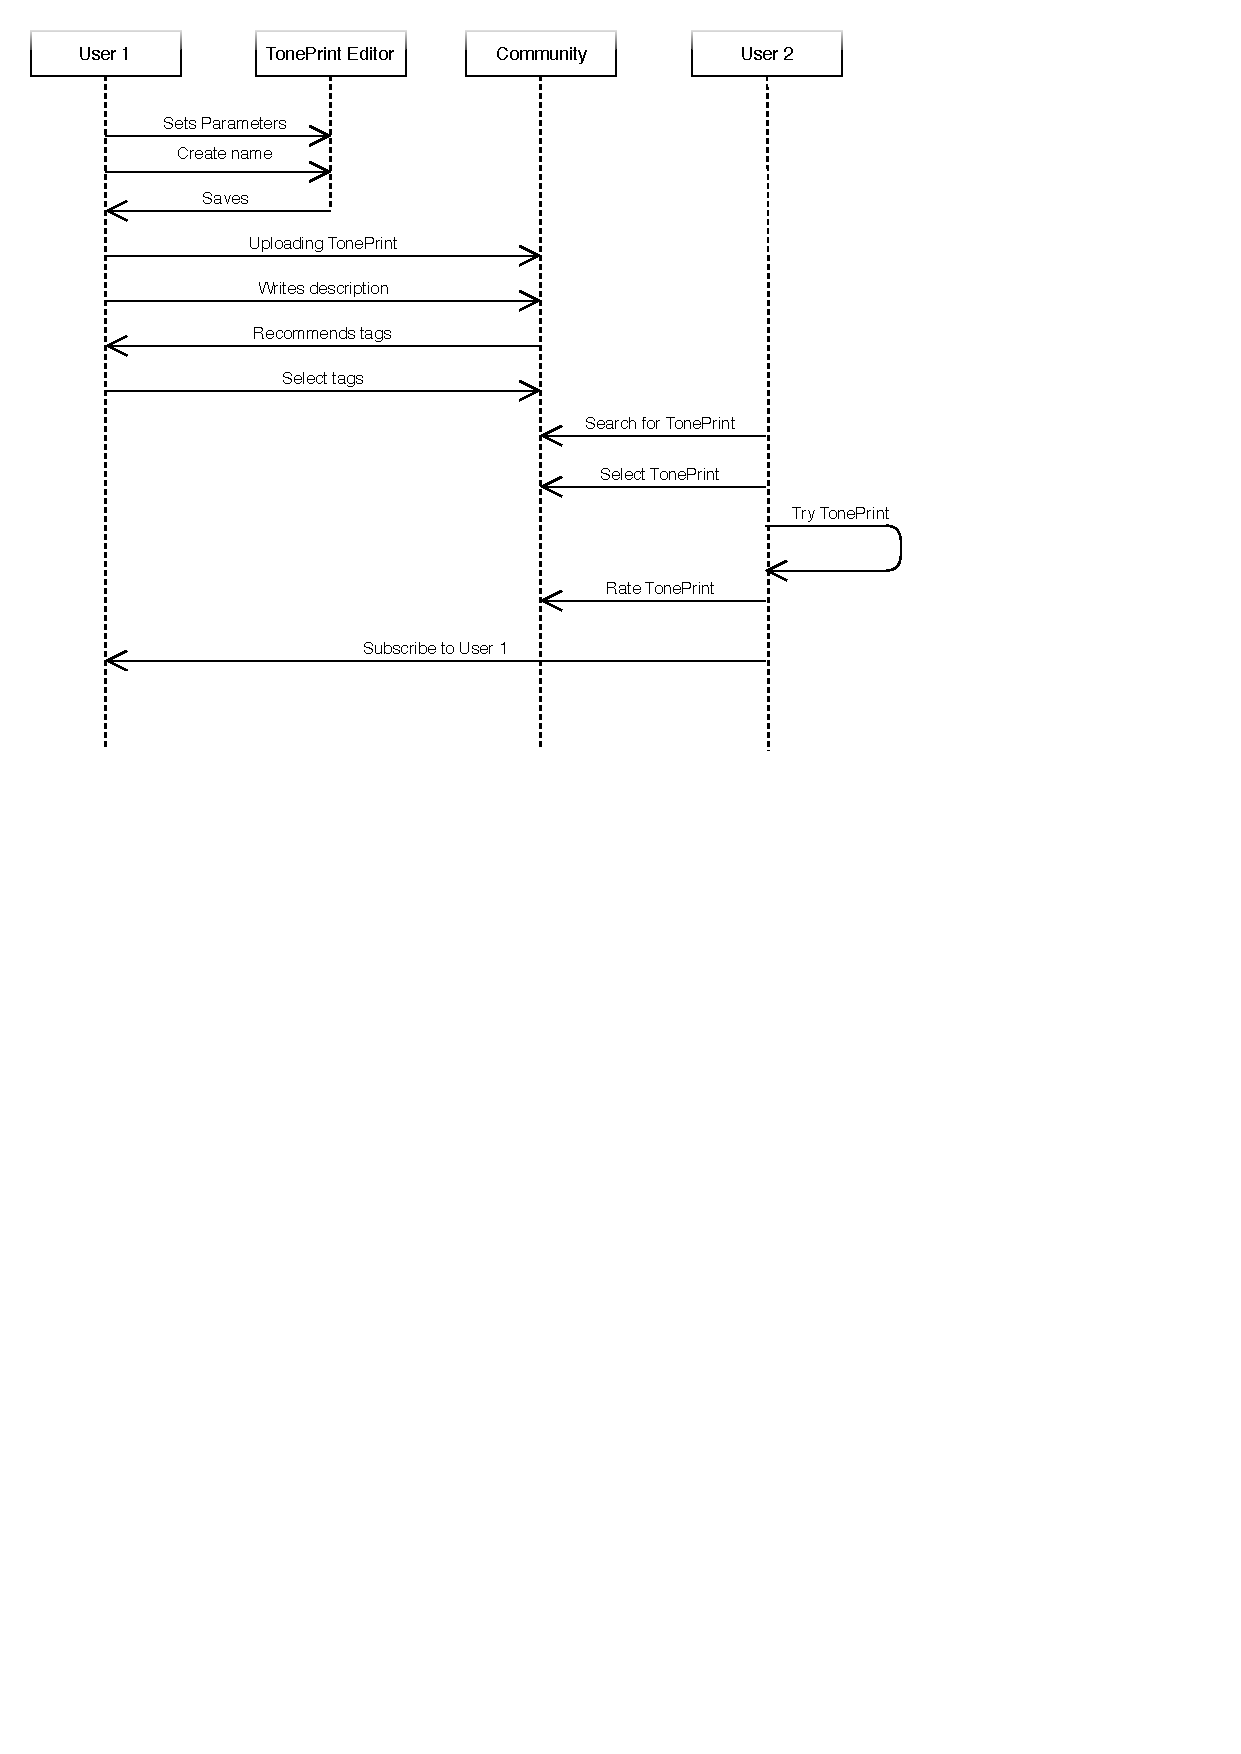
\includegraphics[width=0.95\textwidth]{CommunityUseCaseOne.pdf}
	\caption{a graphical overview of the TonePrint Community use case}
	\label{fig:CommunityConceptualUseCase}
\end{figure}